\documentclass[twocolumn]{article}
\usepackage{graphicx}
%permite ecribir acentos directamente
\usepackage[utf8]{inputenc}
% Esto es para que el LÁTEX sepa que el texto está en español, se agrega el ingles para el paquete de gráfico de circuitos:
\usepackage{float}
\usepackage[spanish]{babel}
\usepackage{geometry}
 \geometry{a4paper,total={170mm,257mm},left=10mm,right=10mm,top=15mm,bottom=15mm}
\usepackage{hyperref} 
\usepackage{amsmath, amsfonts}
\usepackage{enumitem}
\usepackage{xcolor}
\usepackage{textcomp}
\usepackage{fancyhdr}
\usepackage{multicol}

\pagestyle{fancy}
\fancyhf{}
\lhead{Electrónica Aplicada III}
\rhead{TP4:PLL}
\rfoot{Página \thepage}

\usepackage{pgfplots}
\usepackage{pgfplotstable}
\usepackage{booktabs}
\usepackage{array}
\usepackage{colortbl}

\usetikzlibrary{intersections}
\usepackage{siunitx}

\usepackage{booktabs,caption}
\usepackage[flushleft]{threeparttable}

\pgfplotstableset{% global config, for example in the preamble
  every head row/.style={before row=\toprule,after row=\midrule},
  every last row/.style={after row=\bottomrule},
  fixed,precision=1,
}

\usepackage{tikz,pgfplots}            

\pgfplotsset{compat=1.12}
\usetikzlibrary{intersections}

\tikzset{
    every pin/.style={font=\tiny, outer sep=0},
    every pin edge/.style={gray,very thin,shorten >=-1mm},
    small dot/.style={fill=black,circle,scale=0.3}
}

\usepackage{adjustbox}

\begin{document}
\begin{titlepage}
 \centering
	
\includegraphics[scale=0.80]{imagenes/LOGO.jpg} \par
 	\vspace{1cm}
 	{\scshape\LARGE Universidad Tecnológica Nacional \par}
 	{\scshape\large Facultad Regional de Córdoba \par}
 	\vspace{1cm}
	{\bfseries \Large Trabajo Práctico De Laboratorio $N^{\circ} 4$\par}
	{\bfseries \Large Phase Locked Loop (PLL)\par}
 	\vspace{1.5cm}

	\begin{tabular}{ll}
		Alassia, Francisco	&	60861	\\
		Amaya, Matías		&	68284	\\
		Lamas, Matías 		&	65536 	\\
		Navarro, Facundo 	&	63809 	\\
		Veron, Misael	 	&	62628
	\end{tabular}
	
	\vspace{1cm}
	Curso: 5r2 \\
	Grupo $N^{\circ} 4$
 	\vfill
	{\bfseries \Large Electrónica Aplicada III \par}

	\vspace{1.5cm}
	Docentes: \par
	Ing. Rabinovich, Daniel \par
	Ing. Yoaquino, Leandro \par

 	\vfill
	{\large \today\par}
\end{titlepage}

%##################################### INDICE  #####################################################
\onecolumn
\tableofcontents
\clearpage

%##################################### INDICE  #####################################################
\twocolumn
\section{Introducción}
Un ``Phase Locked Loop" ($PLL$) o bucle de fase enganchado consta de una serie de bloques interconectados que le permiten al sistema ajustarse y modificar su frecuencia hasta que no exista diferencia de fase entre las señales de entrada y salida. Es un sistema de control realimentado, donde la señal de realimentación es una frecuencia en lugar de una tensión. 

Se lo conoce también como sintetizador de frecuencia, ya que permite disponer de una frecuencia muy estable y precisa.

Sus principales aplicaciones son:
\begin{itemize}\itemsep0em
	\item Generación y recuperación de portadoras en emisión.
	\item Demodulación de señales analógicas o digitales moduladas en frecuencia. 
	\item Divisores y multiplicadores de frecuencia.
\end{itemize}

El $PLL$ tiene dos modos de operación,
\begin{itemize}
	\item \textbf{\textit{Modo de Adquisición}} donde el $PLL$ intenta sincronizar la frecuencia y la fase de salida del $VCO$ con una señal de entrada. En este modo el $PLL$ se comporta como un sistema no lineal y los errores de fase entre las señales puede ser grande.
	\item \textbf{\textit{Modo de Seguimiento}} donde el $PLL$ se puede estudiar como un sistema lineal simple y la diferencia de fase entra las señales de entrada y salida es pequeña. 
\end{itemize}

\section{Marco Teórico}
\subsection{Estados de funcionamiento}
\begin{itemize}
	\item \textit{Estado dinámico}: Cuando la salida no está enganchada o sincronizada con la referencia. Como un caso particular de este caso se encuentra el estado de ``corrida libre".
	\item \textit{Estado estático}: Corresponde cuando la salida está enganchada o sincronizada con la referencia. También se denomina estado fijo. 
\end{itemize}

\subsection{Bloques y principio de funcionamiento}
En la figura \textcolor{blue}{{\ref{fig:fig1}}} se muestra un diagrama en bloques que representa la estructura básica de un circuito $PLL$.

\begin{figure}[H]
  \centering    
  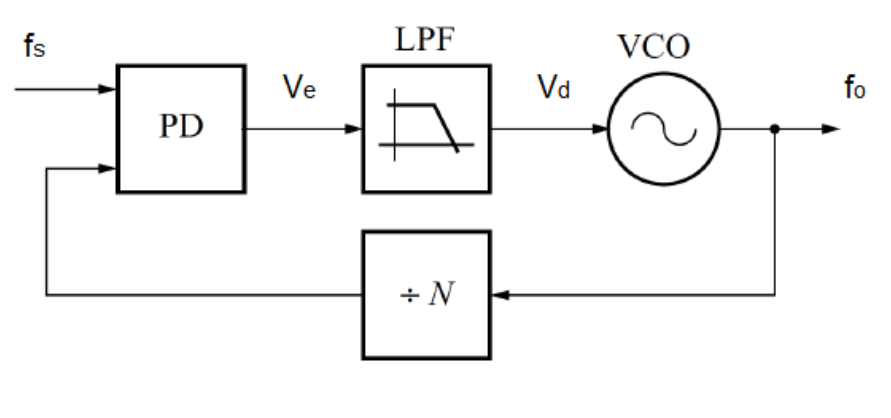
\includegraphics[width=\columnwidth]{imagenes/fig1.jpg}
	\caption{Bloques principales de un $PLL$.}\label{fig:fig1}
\end{figure}

\begin{itemize}
	\item \textit{Comparador de fase} 
		El comparador de fase es un dispositivo no lineal con dos señales de entrada cuya frecuencia son $fs$ y $f_O/N$, generalmente es un mezclador. La salida de este bloque contiene la suma y diferencia de las frecuencias de entrada, es el filtro pasa bajos el que se encarga de que solo se transmita la señal diferencia, que es una tensión continua cuando el $PLL$ se encuentra enganchado.

La salida genera una tensión que es función de la diferencia de fase $\theta_e = \theta_s - \theta_n$ entre las señales de entrada. Si la frecuencia de entrada es igual a la frecuencia de corrida libre del $VCO$, la tensión de control deberá ser cero. En los comparadores de fase más comunes, la tensión de salida es función sinusoidal, triangular o diente de sierra de la diferencia de fase.

	El factor de ganancia del comparador de fase en estado enganchado se expresa como,
	\[ K_d = \frac{\Delta V_e}{\Delta \theta_e} \]

  \item \textit{Filtro pasa bajos} 

	  El filtro pasa bajos tiene dos funciones principales,
	\begin{itemize}
	  \item En primer lugar, eliminar ruido y componentes de alta frecuencia, dejando pasar solo la diferencia $f_s - f_n$ o una tensión continua cuando el lazo está fijo y estable.
	  \item En segundo lugar, este es el bloque que más influye en la determinación de las características dinámicas del lazo, como el rango de captura y enganche, el ancho de banda y la respuesta transitoria.
	\end{itemize}
El filtro puede ser activo o pasivo, en el presente se emplea un filtro $RC$ cuya función de transferencia es la siguiente,
$$ F(s) = \frac{1}{1 + \tau s} $$

\item \textit{Oscilador controlador por tensión} 

	EL $VCO$ (oscilador controlado por tensión) tiene una frecuencia de corrida libre $f_f$ y un desplazamiento de frecuencia de $\Delta f_O$ que es proporcional a la tensión de entrada $V_d$. La frecuencia de salida se puede expresar como:
\[ f_O = f_f + \Delta f_O = f_f + K_O V_d \]

La relación entre el corrimiento de la frecuencia de salida con el corrimiento de la fase de salida está dada por la siguiente relación:
\[ \theta_O (s) = K_O \frac{V_d}{s} \]
Analizando el funcionamiento, el $VCO$ oscila libremente a una frecuencia $f_f$, llamada \textit{frecuencia de corrida libre}. La cual es comparada con la frecuencia $f_s$, llamada \textit{frecuencia de referencia}, en el comparador de fase. El filtro, que es del tipo pasa bajos, se encarga de eliminar las componentes de alta frecuencia. Si la frecuencia de la señal de salida del bloque de filtrado $V_e$ es suficientemente baja, el filtro no la atenúa, entonces $V_d$ controla el $VCO$ tendiendo a reducir la diferencia entra las frecuencias hasta que se igualen.

Una vez que las señales de entrada y salida se igualan, es decir $f_o = f_s$, el detector de fase entrega una tensión con una componente continua estable para que el $VCO$ iguale la frecuencia de la señal de referencia.

El $VCO$ actúa como un integrador de los errores de fase. Mantiene el estado fijo del bucle durante perturbaciones momentáneas.
\end{itemize}

\subsection{Rangos de funcionamiento}
\begin{itemize}
	\item \textit{Corrida libre}: Corresponde a la frecuencia de salida $fo$ del $VCO$ cuando el $PLL$ no se encuentra enganchado.
	\item \textit{Rango de sostén}: Rango en el cual el $PLL$ puede mantener el ``tracking" o seguimiento de fase. El $PLL$ está enganchado con la señal de referencia si ésta se reduce o incrementa lentamente. Si, en cambio, varía mucho, el $PLL$ puede perder el enganche en los extremos.

	\item \textit{Rango de captura}: A partir del $PLL$ desenganchado, es el rango de frecuencias en el que el mismo puede engancharse a la frecuencia de entrada. Este define el rango de operación del $PLL$.
\end{itemize}

\begin{figure}[H]
  \centering    
  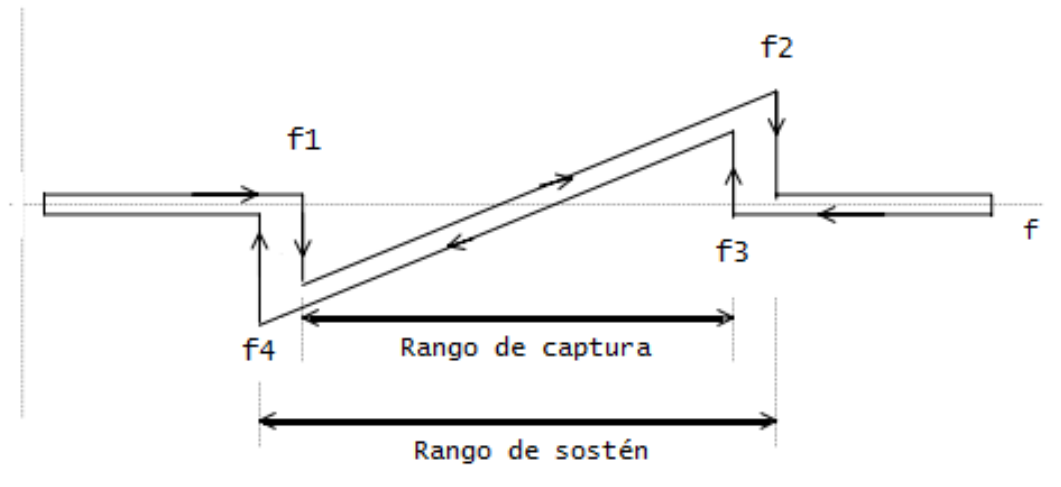
\includegraphics[width=\columnwidth]{imagenes/fig0.jpg}
	\caption{Rangos de funcionamiento.}\label{fig:fig0}
\end{figure}

En la figura \textcolor{blue}{{\ref{fig:fig0}}} se pueden observar los rangos mencionados anteriormente.

\section{Diseño de red $PLL$}
En esta sección se realizarán los cálculos para la implementación de una red $PLL$ multiplicadora por 10, con las siguientes especificaciones:
\begin{itemize}\itemsep0em
\item $f_o = 15 kHz \; a  \; 25kHz $
	\item $\xi = 0.4$
	\item $V_{DD} = 12 V$
	\item Filtro de lazo $RC$
\end{itemize}

El circuito se diseña en Kicad, a continuación en las imaginen \textcolor{blue}{{\ref{fig:sch}}} presenta el esquemático yen la imagen \textcolor{blue}{{\ref{fig:pcb1}}}, el PCB.
\begin{figure}[H]
  \centering    
  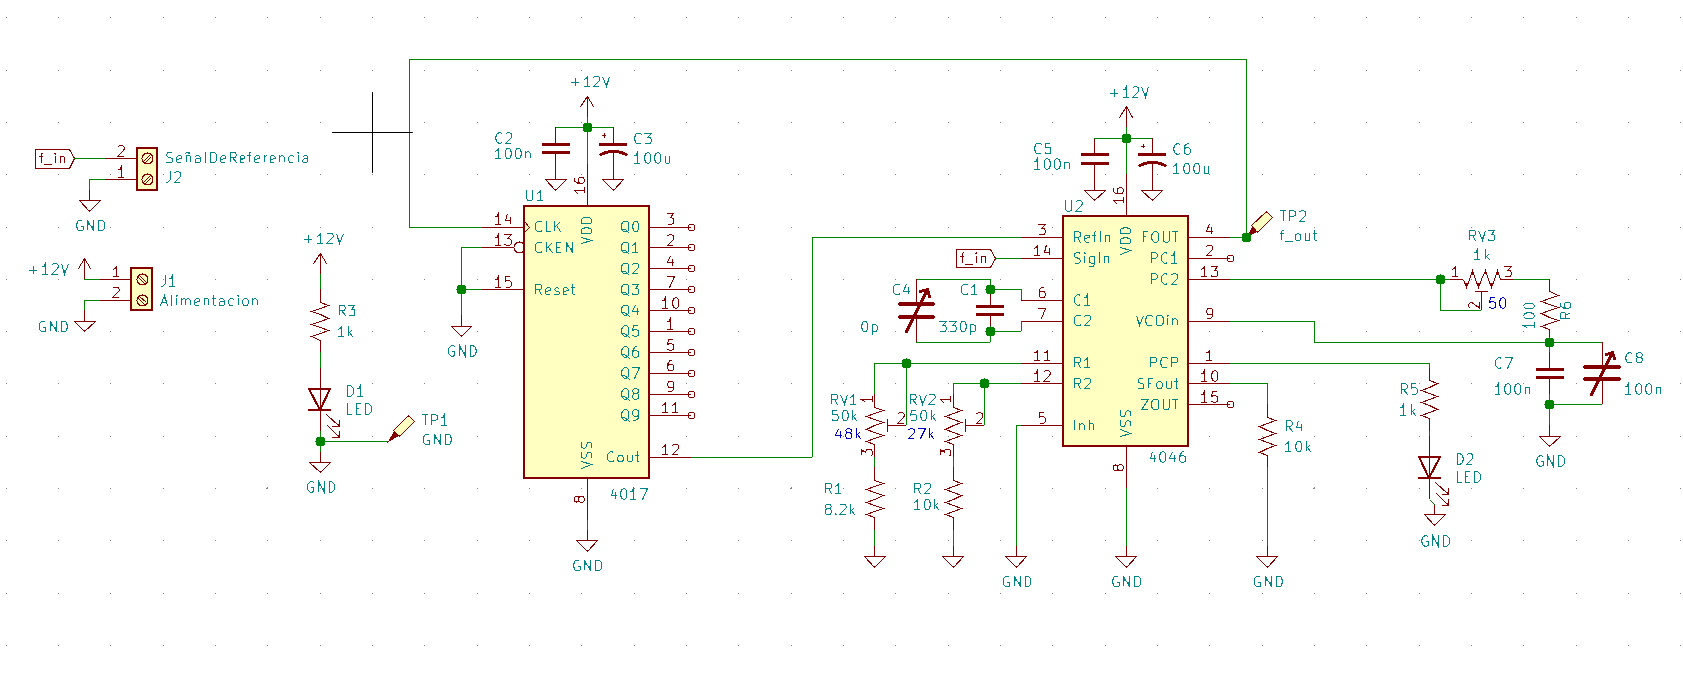
\includegraphics[width=\columnwidth]{imagenes/sch.jpg}
	\caption{Esquemático realizado en Kicad.}\label{fig:sch}
\end{figure}

\begin{figure}[H]
  \centering    
  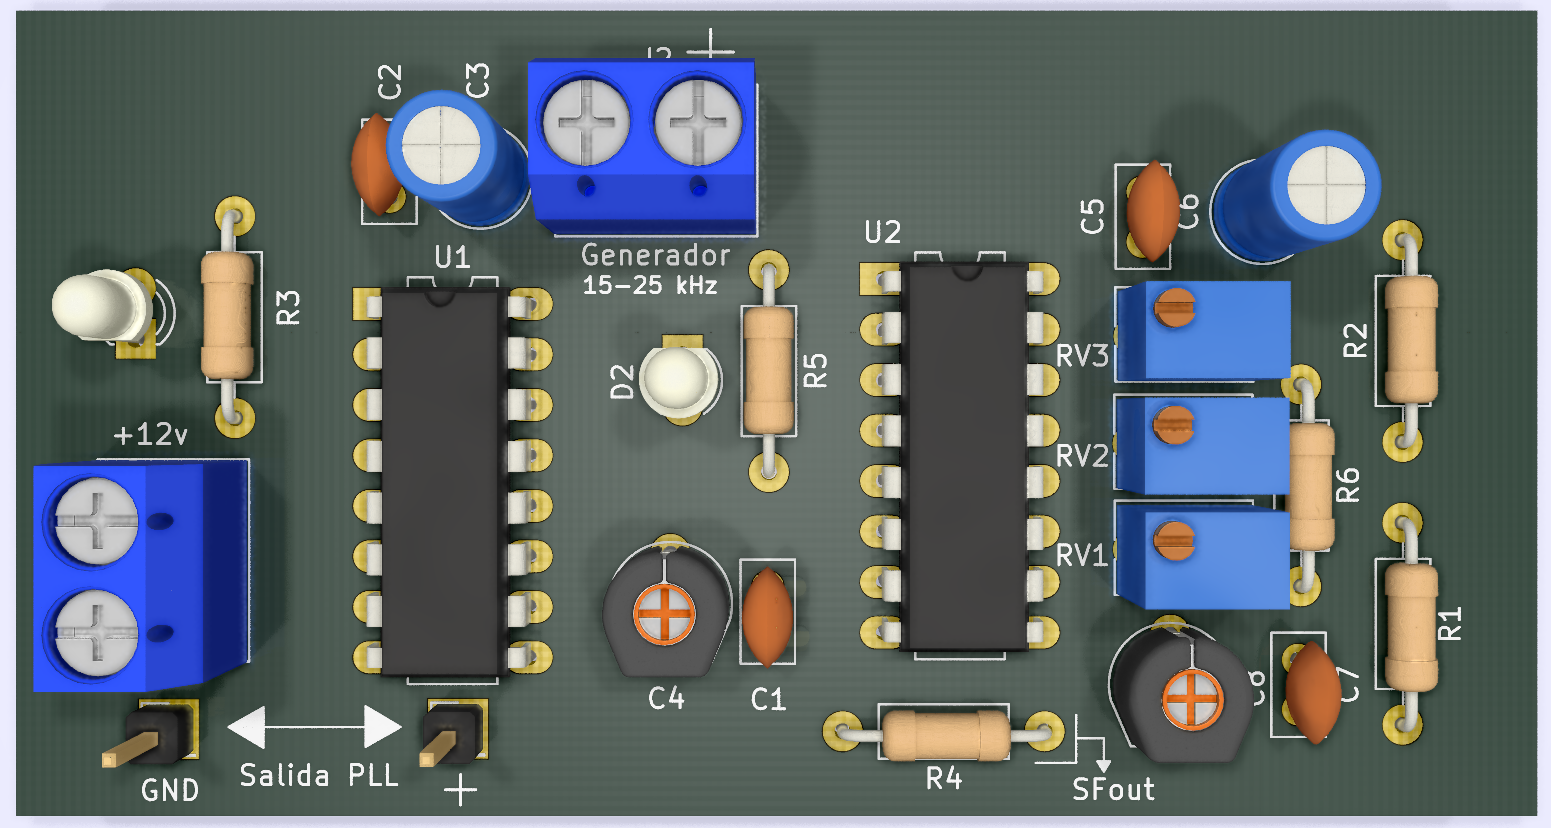
\includegraphics[width=\columnwidth]{imagenes/pcb1.jpg}
	\caption{Render PCB en Kicad}\label{fig:pcb1}
\end{figure}

\subsection{Cálculos de componentes}
En la hoja de datos del integrado $CD4046$ encontramos la relación de $R2/C1$ en la figura \textcolor{blue}{{\ref{fig:fig4}}} y de $R2/R1$ en la figura \textcolor{blue}{{\ref{fig:fig3}}} del dicho datasheet, las cuales se presentan a continuación, 

\begin{figure}[!ht]
  \centering    
  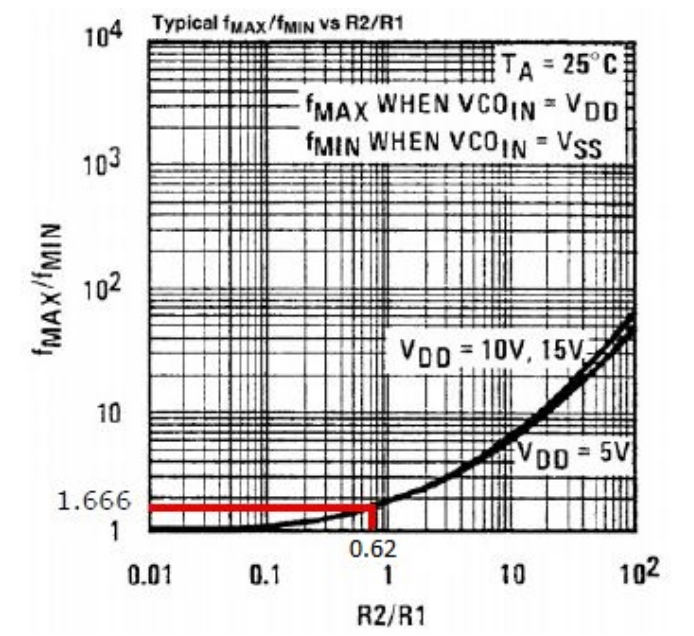
\includegraphics[width=\columnwidth]{imagenes/fig3.jpg}
	\caption{Cálculo de coeficiente $R2/R1$.}\label{fig:fig3}
\end{figure}

\begin{figure}[!ht]
  \centering    
  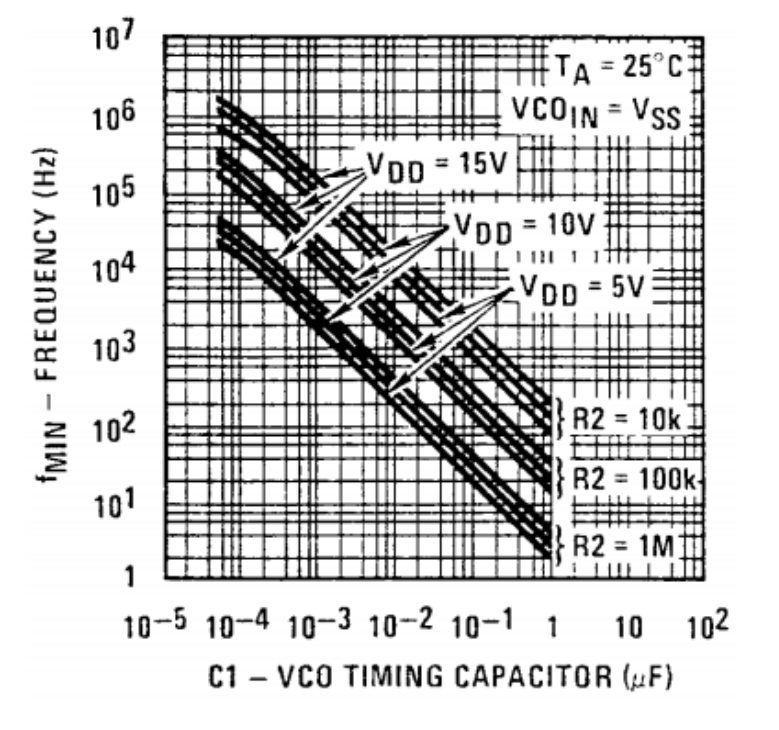
\includegraphics[width=\columnwidth]{imagenes/fig4.jpg}
	\caption{Cálculo de C1 y R2.}\label{fig:fig4}
\end{figure}

\subsubsection{C1 y R2}
Para obtener el valor de $C1$, debemos ubicarnos en la imagen \textcolor{blue}{{\ref{fig:fig4}}}, donde se deberá tener en cuenta la frecuencia mínima de trabajo y la tensión de alimentación de nuestro circuito. 

Eligiendo un valor de $R2$ de $100 \; k \Omega$ se obtiene un valor de $C1$ de aproximadamente 140 $pF$. 

\subsubsection{R1}
Como se visualiza en la figura \textcolor{blue}{{\ref{fig:fig3}}}, la relación de $R2$ con $R1$ está determinada por la frecuencia máxima y mínima de trabajo de dicho $PLL$. De esta manera obtenemos la relación de frecuencias,
\[ \frac{f_M}{f_m} = \frac{250kHz}{150kHz} = 1,666 \]
Por medio de ésto proseguimos a obtener la relación de $R2$ con $R1$ por medio de la tabla, donde 
$$ \frac{R2}{R1} = 0,62 $$

Siendo $R2 \; = \; 100 \; k \Omega$ , entonces $R1$ tendrá un valor de $161,29 \; k\Omega$.

\subsubsection{R3 y C2}

Estos valores dependen de la respuesta transitorio que se desee obtener. Por las condiciones especificadas el valor de coeficiente de amortiguamiento es de $\xi = 0,4$.

Para encontrar el valor numérico de estos componentes es necesario obtener en primer lugar las ganancias $K_d$ y $K_O$,

\begin{figure}[H]
  \centering    
  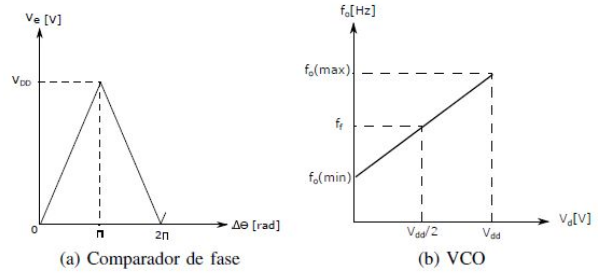
\includegraphics[width=\columnwidth]{imagenes/fig5.jpg}
	\caption{Respuesta del VCO y PD.}\label{fig:fig5}
\end{figure}

La forma de onda de la tensión de salida del comparador de fase empleado se encuentra a la izquierda de la figura \textcolor{blue}{{\ref{fig:fig5}}}. A partir de esta se obtiene $K_d$ según la siguiente relación,
\[ K_d = \frac{\Delta V_E}{\Delta \theta_E} = \frac{V_{DD}}{\pi} = 3,819 \frac{V}{rad} \]

En la figura de la derecha de \textcolor{blue}{{\ref{fig:fig5}}} se muestra una gráfica que relaciona la tensión $V_d$, de entrada al $VCO$, con la frecuencia $f_O$ de salida. La ganancia $K_O$ del $VCO$ se obtiene de la siguiente manera,
\begin{align*}
	K_O &= \frac{2 \pi \Delta f_o}{\Delta V_d} \\
		&= \frac{2 \pi (f_{max} - f_{min})} {V_{DD}} \\
	K_O &= 52359,877 \frac{rad}{s}
\end{align*}

La ganancia de lazo está determinada por
\[ \frac{K_d \cdot K_O}{N} \approx 20000 \]
donde $N$ es el coeficiente de división del bloque divisor.

Por teoría de control se obtiene la relación entre las ganancias calculadas($K_d$,$K_O$), el coeficiente de amortiguamiento ($\xi$), coeficiente de división ($N$) y los valores de $R3$ y $C2$, expresada como 
\[ R_{3} \cdot C_2 = \frac{N}{{(2\xi)}^2 K_d K_O}\]

Tomando un valor de $C2$ de $10nF$ obtenemos el valor correspondiente de $R3$, el cual es de $15,625 k\Omega$

\section{Experiencia práctica}
Finalmente se procedió a realizar el circuito, el cual se muestra en la imagen \textcolor{blue}{{\ref{fig:fig6}}}, para la medición de los rangos se utiliza un generador de funciones de onda cuadrada, con un duty cycle del $50\%$ y una amplitud de 0-$V_{DD}$.

Para facilitar el ajuste general del circuito, se utilizaron resistencias variables.

\subsection{Rangos de funcionamiento}
\begin{figure}[H]
  \centering    
  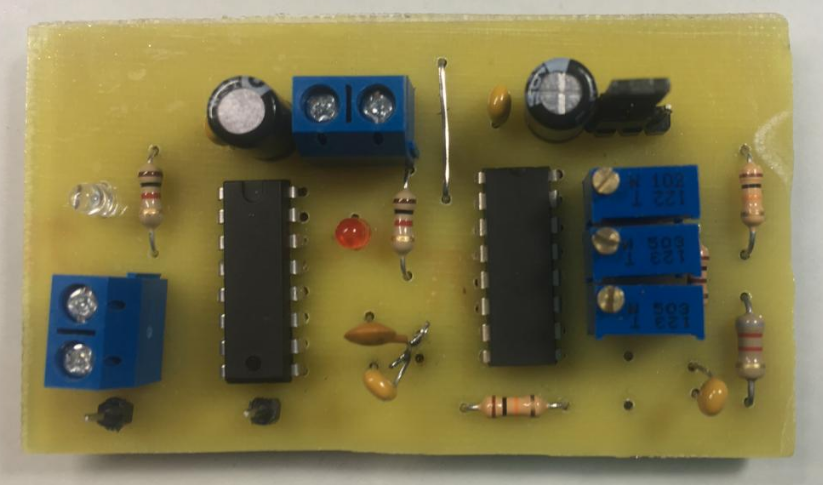
\includegraphics[width=\columnwidth]{imagenes/fig6.jpg}
	\caption{Circuito implementado.}\label{fig:fig6}
\end{figure}

Para la medición del rango de captura, se ajustó la señal de entrada fuera del rango de trabajo, para luego acercarla lentamente por ambos extremos hasta encontrar la frecuencia de ``enganche", si ésta estaba fuera de las especificaciones a través de las resistencias variables $RV1$ y $RV2$ se ajustaban para que estuvieran dentro de los parámetros de diseño.

Luego para el rango de sostén, una vez enganchado el $PLL$ en las frecuencias especificadas, se variaba levemente la frecuencia en los extremos hasta que el sistema perdiera el sincronismo.

A continuación se exponen los resultados.
\begin{itemize}
	\item Rango de captura
		\begin{itemize}
			\item $f_1$ = 
			\item $f_3$ = 
		\end{itemize}
	\item Rango de sostén
		\begin{itemize}
		  \item $f_4$ = 
		  \item $f_2$ =
		\end{itemize}
\end{itemize}

\subsection{Ganancia de lazo}
Para el cálculo de la ganancia de lazo, se mide con un osciloscopio el desfasare entre la señal introducida (pin 14) y la que se obtiene del mismo integrado (pin 3)a dos frecuencias distintas según la condición de que 15 kHz $< f_s > $25 kHz.

\begin{itemize}
	\item \textbf{$f_{s1}: 16 kHz$}
	  \begin{itemize}
		  \item $T_1$ =
		  \item $\tau_1$ =
		  \item $\theta_1$ =
	  \end{itemize}
\end{itemize}


\begin{figure}[H]
  \centering    
  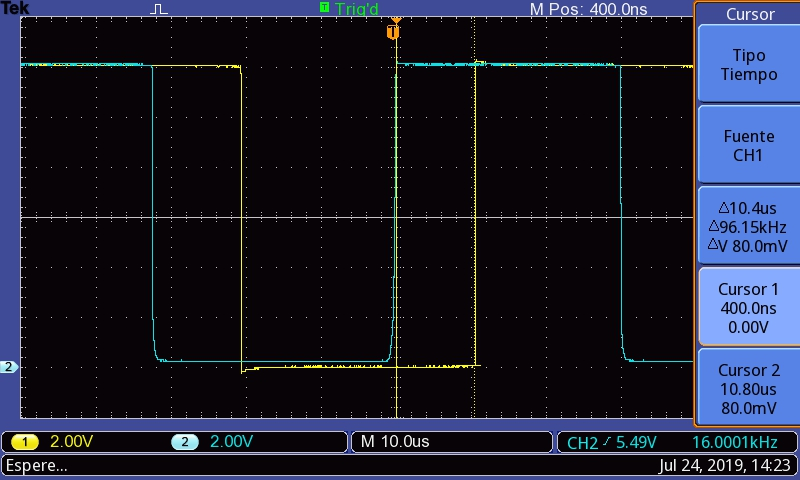
\includegraphics[width=\columnwidth]{imagenes/osc1.jpg}
  \caption{Ganancia de $f_{s1}$.}\label{fig:osc1}
\end{figure}

\begin{itemize}[*]
	\item \textbf{$f_{s2}: 22 kHz$}
	  \begin{itemize}
		  \item $T_2$ =
		  \item $\tau_2$ =
		  \item $\theta_2$ =
	  \end{itemize}
\end{itemize}


\begin{figure}[H]
  \centering    
  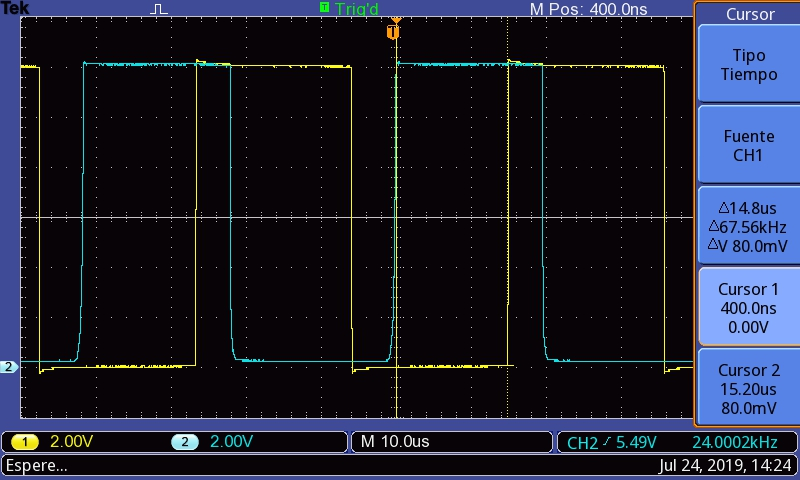
\includegraphics[width=\columnwidth]{imagenes/osc2.jpg}
  \caption{Ganancia de $f_{s2}$.}\label{fig:osc2}
\end{figure}

La ganancia de lazo se puede calcular como hemos visto anteriormente,
\begin{align*}
	\frac{K_o K_d}{N} &= \frac{\Delta \omega s}{\Delta \theta} \\
					  &= \frac{2 \pi (f_{s2} - f_{s1})} {\theta_2 - \theta_1} \\
					  &= 
\end{align*}

\subsection{Sobrepasamiento y constante de tiempo}
Finalmente, el sobrepasamiento se observa al medir la entrada del $VCO$ (voltaje, no frecuencia) para una señal de entrada modulada en frecuencia. La entrada, de 20kHz se modula a 100Hz entre 18kHz y 22kHz, comprobándose previamente que el $PLL$ mantenga el enganche en ese rango.

Como no es posible observar el comportamiento transitorio de la frecuencia de salida lo que se realiza es observar el comportamiento de la tensión $V_d$ a partir de las cuales se obtiene el sobrepasamiento porcentual $M_{p}$.

Por otra parte para la misma forma de onda se determina el tiempo de pico $t_p$. 

\begin{figure}[H]
  \centering    
  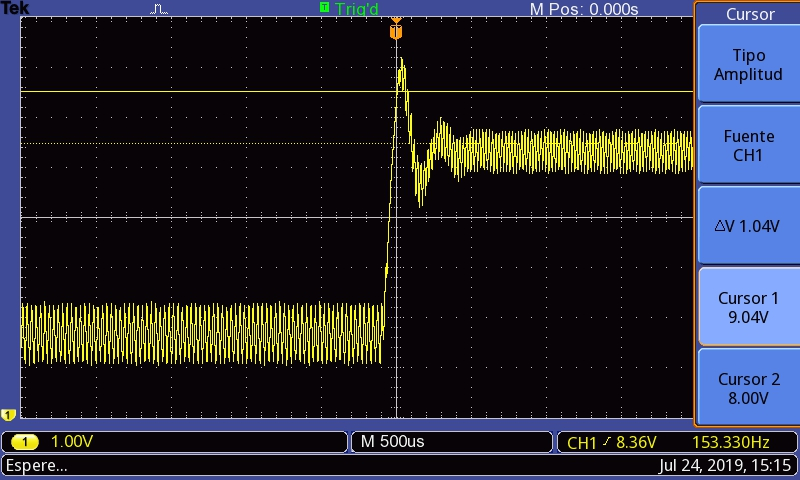
\includegraphics[width=\columnwidth]{imagenes/Ymax.jpg}
  \caption{$Y(max) - Y(\infty)$.}\label{fig:Ymax$}
\end{figure}

\begin{figure}[h]
  \centering    
  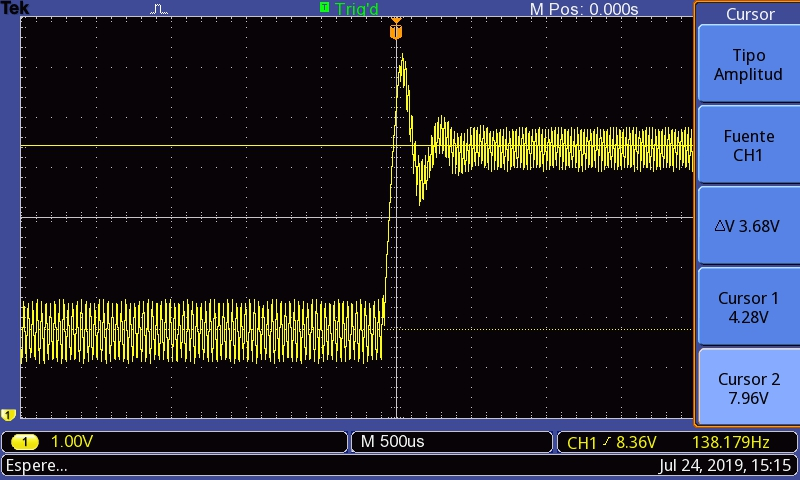
\includegraphics[width=\columnwidth]{imagenes/Yinf.jpg}
  \caption{$Y(\infty)$}\label{fig:Yinf}
\end{figure}

\begin{figure}[h]
  \centering    
  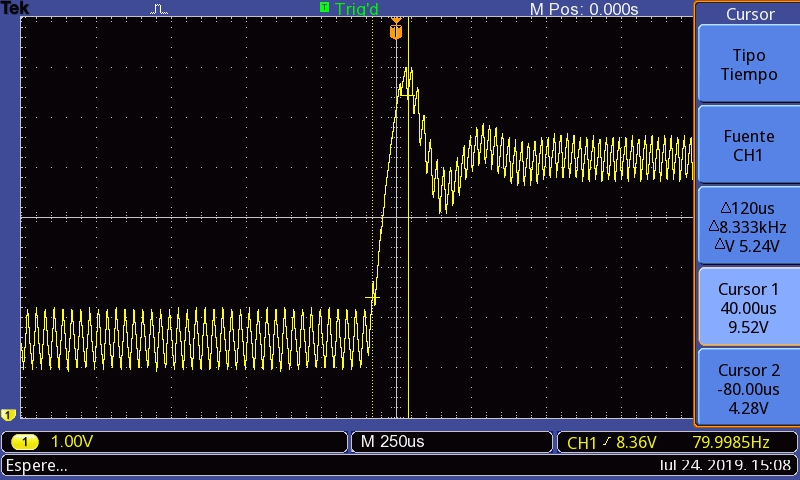
\includegraphics[width=\columnwidth]{imagenes/tp.jpg}
  \caption{Tiempo de pico($t_{p}$)}\label{fig:tp}
\end{figure}

De dicha medición se obtuvo el valor de $t_p = $ $us$. Con las mediciones obtenidas se procede a calcular el $M_p$.
\[ M_p = \frac{Y(max) - Y(\infty)} {Y(\infty)} * 100 \]

Obtenido el $M_p$ se procede a calcular el $\xi$ de nuestro $PLL$. Donde recordamos que,
\[ \xi = \frac{\sigma}{\omega n} \]

Para la obtención de $\sigma$ despejamos de esta variable de la ecuación \textcolor{blue}{\ref{eq1}}
\begin{equation}
	M_{p} = e^{-\frac{\pi \sigma}{\omega_{n}}}
	\label{eq1}
\end{equation}

Para esto necesitamos de la relación $\omega_{p}$
\[
	\omega_{p} = \frac{\pi}{t_{p}}
\] 

De la cual podemos explicitar,
\begin{align*}
	\sigma &= - \frac{\omega_{p} \cdot \ln({M_{p})}}{\pi} \\
		   &= - \frac{\ln(M_{p})}{t_p}\\
	\sigma &=    
\end{align*}

Con $\sigma$ calculado, se obtiene $\omega_{n}$ según lo siguiente,
\begin{align*}
	\omega_{n} &= \sqrt{{\omega_{n}}^{2}+ {\sigma}^{2}} \\
	\omega_{n} &=
\end{align*}

Finalmente obtenemos $\xi$,

\begin{align*}
  \xi &= \frac{\sigma}{\omega_{n}} \\
      &= \frac{}{} \\
  \xi &=
\end{align*}

Como podemos comprobar el valor obtenido es similar al dado por la condición de diseño ($\xi = 0,4$).
 
\section{Conclusión}
El cálculo de los componentes de la red se realiza según las especificaciones indicadas en el práctico, empleando la hoja de datos proporcionada por el fabricante del integrado $CD4046$, donde se hace uso de gráficas para la obtención de las magnitudes a implementar, por lo que la exactitud de éstas no es muy buena.

Este es uno de los motivos por el cual en el momento de implementar nuestro $PLL$, los valores calculados durante el desarrollo de este informe debieron ser modificados, y éstos quedaron determinados a prueba y error de los integrantes del grupo para que dicho $PLL$ trabaje en la zona deseada.

Por último, si el comportamiento transitorio del $VCO$ no es el adecuado, se puede modificar mediante la variación de los parámetros del bloque de filtrado.

A continuación se mostrará una tabla informativa con los valores obtenidos mediante cálculos y aquellos valores que fueron usados para la implementación y buen funcionamiento del $PLL$.

\begin{table}[H]
\centering
\begin{tabular}{|l|l|l|}
\hline
						 & Cálculos & Implementación \\ \hline
R1                       &          &                \\ \hline
R2                       &          &                \\ \hline
R3                       &          &                \\ \hline
C1                       &          &                \\ \hline
C2                       &          &                \\ \hline
\end{tabular}
\end{table}

\end{document}

